% ================================================================
%  FuzzyShield — IEEE Conference Paper Format
%  Compile: pdflatex main.tex  (run twice for refs)
% ================================================================
\documentclass[conference]{IEEEtran}
\IEEEoverridecommandlockouts
% The preceding line is only needed to identify funding in the first footnote.

\usepackage{cite}
\usepackage{amsmath,amssymb,amsfonts}
\usepackage{algorithmic}
\usepackage{graphicx}
\usepackage{textcomp}
\usepackage{xcolor}
\usepackage{booktabs}
\usepackage{array}
\usepackage{multirow}
\usepackage{tabularx}
\usepackage{float}
\usepackage{listings}
\usepackage{enumitem}
\usepackage[utf8]{inputenc}
\usepackage{hyperref}

\def\BibTeX{{\rm B\kern-.05em{\sc i\kern-.025em b}\kern-.08em
    T\kern-.1667em\lower.7ex\hbox{E}\kern-.125emX}}

\lstset{
  basicstyle      = \ttfamily\scriptsize,
  keywordstyle    = \bfseries,
  numbers         = left,
  numberstyle     = \tiny,
  numbersep       = 5pt,
  breaklines      = true,
  showstringspaces= false,
  captionpos      = b,
  frame           = single,
}

\begin{document}

\title{FuzzyShield: Real-Time Behavioral Malware\\Classification Using Fuzzy Logic%
\thanks{Term Project Report --- Introduction to Artificial Intelligence,
Dept.\ of Computer Engineering, Izmir Institute of Technology, June 2026.}}

\author{\IEEEauthorblockN{Ahmet Faruk Kesgin}
\IEEEauthorblockA{\textit{Dept. of Computer Engineering} \\
\textit{Izmir Institute of Technology}\\
Urla, Izmir, Türkiye \\
{[300201024]}}}

\maketitle

\begin{abstract}
This project proposes a fuzzy logic system to classify malware based on
real-time behaviors (CPU, file I/O, and network traffic) rather than
static signatures. It calculates the probability of a process being
Ransomware, a Trojan, or a Cryptominer to defend against zero-day
attacks.

The system collects ten behavioral metrics from a running process, applies
a Mamdani fuzzy inference engine with 34 expert-defined rules, and
produces three independent threat scores through centroid defuzzification.
A compound-threat verdict mechanism reports co-occurring threats when
multiple scores exceed a minimum activation threshold. The system is
implemented in both Python (scikit-fuzzy) and MATLAB (Fuzzy Logic
Toolbox) with an exact one-to-one rule correspondence between both
environments. Experimental evaluation across five preset scenarios
demonstrates correct high-confidence classification: Ransomware at
$83.5\%$, Trojan at $76.3\%$, Cryptominer at $83.7\%$, and Benign at
$6.6\%$. A mixed scenario simultaneously triggering ransomware-like
file-write patterns and trojan-like network exfiltration produces a
compound \textit{RANSOMWARE\,+\,TROJAN} verdict, demonstrating the
system's ability to handle ambiguous real-world attack profiles.
In real-time process monitoring, an asymmetric exponential weighted
moving average (EWMA) with $\alpha_{\uparrow}{=}0.15$ (fast rise) and
$\alpha_{\downarrow}{=}0.85$ (slow fall) smooths consecutive inference
scores to neutralise burst-pause evasion attempts.
\end{abstract}

\begin{IEEEkeywords}
fuzzy logic, malware detection, behavioral analysis, Mamdani inference,
ransomware, trojan, cryptominer, zero-day
\end{IEEEkeywords}

% ════════════════════════════════════════════════════════════════════════════
\section{Introduction}

Modern operating systems are constantly targeted by sophisticated malware
that exploits vulnerabilities before security patches become available ---
so-called \textit{zero-day} attacks. Traditional antivirus tools depend
on signature databases: a binary hash, a byte sequence, or a known code
pattern must be catalogued before a sample can be detected. This reactive
approach is fundamentally ill-suited to novel threats, since a zero-day
sample by definition has no prior signature.

Behavioral analysis offers a complementary strategy: instead of inspecting
the static content of an executable, the system observes what a running
process \emph{does} --- how aggressively it consumes CPU, how much it reads
and writes to disk, how many files it encrypts, and whether it establishes
unusual network connections. Malware families exhibit characteristic
behavioral footprints: ransomware writes large amounts of high-entropy
(encrypted) data to many different file types; trojans maintain persistent
outbound connections and exfiltrate data; cryptominers saturate CPU cores
while sending structured, low-entropy traffic to mining pool servers.

Behavioral metrics are inherently imprecise. A CPU load of $78\%$ is
neither unambiguously ``normal'' nor unambiguously ``malicious''; it
occupies a \emph{fuzzy} grey zone. Fuzzy logic~\cite{zadeh1965} was
designed exactly for this kind of uncertain, overlapping classification
problem. By encoding behavioral expertise as IF--THEN rules over
linguistic variables (e.g., ``IF file-write-rate is \textit{extreme}
AND entropy is \textit{max} AND file-extensions are \textit{many} THEN
ransomware risk is \textit{critical}''), the system can reason over
continuous sensor readings without requiring hard thresholds.

This project presents \textbf{FuzzyShield}, a Mamdani fuzzy inference
system that classifies running processes into three malware categories ---
Ransomware, Trojan, and Cryptominer --- by monitoring ten real-time
behavioral metrics. The main contributions are:

\begin{enumerate}[leftmargin=1.8em]
  \item A 10-input, 3-output Mamdani FIS with 34 expert-crafted rules
        covering single-threat, mixed-threat, and benign behavioral
        patterns.
  \item A compound-threat verdict mechanism that reports multiple co-active
        threat types rather than forcing a single winner.
  \item Dual implementations in Python (scikit-fuzzy) and MATLAB (Fuzzy
        Logic Toolbox) with identical rule bases for cross-validation.
  \item A behavioral malware simulator for live demonstration of all three
        malware types.
  \item An asymmetric EWMA temporal feedback module that raises threat
        scores rapidly when a new signal appears ($\alpha_{\uparrow}=0.15$)
        but decays them slowly ($\alpha_{\downarrow}=0.85$), preventing
        malware from evading detection by alternating brief bursts of
        activity with idle windows.
\end{enumerate}

% ════════════════════════════════════════════════════════════════════════════
\section{Background and Related Work}

\subsection{Malware Behavioral Profiles}

\textbf{Ransomware} encrypts victim files and demands a ransom for the
decryption key. Its behavioral signature is distinctive: it reads each
victim file, overwrites it with ciphertext (producing maximum Shannon
entropy), and cycles through as many file types as possible. I/O rates
of tens to hundreds of MB/s are common, and encryption is typically
performed symmetrically on random-per-session keys, meaning the output
bytes are computationally indistinguishable from random
data~\cite{kharaz2016unveil}.

\textbf{Trojans} masquerade as benign applications while conducting
covert activities, most commonly data exfiltration. Their behavioral
signature centers on network activity: many persistent outbound connections
transmit collected data to command-and-control (C2) servers. File I/O
is modest (reading local data), and CPU is moderate since the bottleneck
is the network~\cite{egele2012survey}.

\textbf{Cryptominers} perform continuous proof-of-work computations,
typically SHA-256 hashing. They maximise all CPU cores (often reaching
$100\%$ utilization), consume large amounts of memory for DAG/hash tables,
and maintain a small set of persistent TCP connections to pool servers.
File I/O is negligible, and pool communication uses structured binary
protocols with low entropy~\cite{gomes2021detecting}.

\subsection{Fuzzy Logic and the Mamdani Inference Engine}

A Fuzzy Inference System (FIS) maps crisp input values to crisp output
values through three stages: \textit{fuzzification},
\textit{rule evaluation}, and \textit{defuzzification}.

\textbf{Fuzzification.} Each crisp input $x_i$ is mapped to membership
degrees $\mu_{A_{ij}}(x_i) \in [0,1]$ for each linguistic term $A_{ij}$
using membership functions (trapezoidal or triangular in this work).

\textbf{Rule evaluation.} A Mamdani rule has the form
\[
  \text{IF } x_1 \in A_{1k} \text{ AND } \cdots \text{ AND }
  x_n \in A_{nk}
  \text{ THEN } y \in B_k
\]
The firing strength of rule $k$ is computed using the \textit{min}
T-norm: $\alpha_k = \min_i \mu_{A_{ik}}(x_i)$. The consequent fuzzy
set is clipped at $\alpha_k$: $\mu'_{B_k}(y) = \min(\alpha_k,\,\mu_{B_k}(y))$.
All fired rules are aggregated using the \textit{max} S-norm:
$\mu_{\text{agg}}(y) = \max_k \mu'_{B_k}(y)$.

\textbf{Defuzzification.} The centroid (centre of gravity) method
converts the aggregated fuzzy set back to a crisp score:
\[
  y^* = \frac{\int y\,\mu_{\text{agg}}(y)\,dy}
             {\int \mu_{\text{agg}}(y)\,dy}
\]

The Mamdani model was chosen over Takagi-Sugeno (TSK) because it supports
rich output membership functions that naturally encode linguistic threat
levels (none, trace, low, medium, high, critical), making the inference
transparent and interpretable by security analysts.

\subsection{Related Work}

Kolbitsch et al.~\cite{kolbitsch2009} demonstrated that system call
sequences alone can fingerprint malware families with high accuracy but
require kernel-level instrumentation. Rieck et al.~\cite{rieck2011}
applied machine-learning to API-call frequency vectors; while accurate,
these approaches lack interpretability --- a neural network does not
explain \emph{why} a process is malicious.

Alazab et al.~\cite{alazab2012} used fuzzy rules on system resource
metrics but limited the rule base to five inputs and two threat
categories. Mosli et al.~\cite{mosli2017} extended fuzzy classification
to network-flow features but did not address real-time per-process
monitoring. FuzzyShield extends these approaches
with a wider metric set (10 inputs), three simultaneous output channels,
a compound-threat verdict, and dual-platform verification.

% ════════════════════════════════════════════════════════════════════════════
\section{System Design}

\subsection{Architecture Overview}

Figure~\ref{fig:arch} shows the FuzzyShield pipeline. A monitoring
process collects behavioral metrics from a target PID using the
\texttt{psutil} library (Linux \texttt{/proc} interface), extracts a
10-dimensional feature vector, and passes it to the FIS. The FIS applies
fuzzification, evaluates all applicable rules, aggregates the consequents,
and defuzzifies three output channels. In real-time monitoring mode, the
three raw FIS scores are passed through an asymmetric EWMA temporal
smoothing module before reaching the verdict module; in single-shot
scenario mode, raw scores are used directly. The verdict module converts
the (smoothed or raw) scores to a human-readable classification with
confidence level.

\begin{figure*}[!t]
  \centering
  
\includegraphics[width=\textwidth]{figures/fig_architecture.png}
  \caption{FuzzyShield system architecture: from raw process metrics
           to compound threat verdict.}
  \label{fig:arch}
\end{figure*}

\subsection{Input Variables and Behavioral Metrics}

Ten behavioral metrics are sampled over a configurable interval
(default: 5 seconds) to capture both instantaneous state and rate-based
activity. Table~\ref{tab:inputs} describes each metric.

\begin{table*}[!t]
\centering
\caption{FuzzyShield Input Variables}
\label{tab:inputs}
\renewcommand{\arraystretch}{1.3}
\begin{tabularx}{\textwidth}{
  >{\ttfamily\small}l
  l
  l
  >{\small}X
}
\toprule
\normalfont\textbf{Variable} & \textbf{Range} & \textbf{Linguistic Terms} & \textbf{Description} \\
\midrule
cpu       & 0--100\%         & idle / low / moderate / high / extreme    & CPU utilization \\
mem       & 0--2048 MB       & tiny / small / medium / large / huge      & Resident set size \\
fwrite    & 0--200 MB/s      & none / low / moderate / high / extreme    & File write rate (wchar) \\
file\_read & 0--200 MB/s     & none / low / moderate / high / extreme    & File read rate \\
nettx     & 0--10000 KB/s    & silent / low / moderate / high / flood    & Network bytes transmitted \\
netrx     & 0--10000 KB/s    & silent / low / moderate / high / flood    & Network bytes received \\
ext       & 0--50            & single / few / several / many / mass      & Unique file extensions accessed \\
conn      & 0--500           & none / few / moderate / many / swarm      & Active TCP connections \\
ent       & 0--8 bits/byte   & ordered / low / medium / high / max       & Shannon entropy of writes \\
priv      & 0--20            & none / low / moderate / high / extreme    & Privilege escalation attempts \\
\bottomrule
\end{tabularx}
\end{table*}

\subsubsection{Shannon Entropy of Write Output}

File-write entropy is sampled by reading the tail bytes of recently
written files and computing:
\[
  H = -\sum_{b=0}^{255} p_b \log_2 p_b
\]
where $p_b$ is the empirical probability of byte value $b$.
High-entropy output ($H \approx 8$) is characteristic of
cryptographically random (encrypted) data; low entropy ($H < 3$)
indicates structured or text data.

\subsection{Output Variables}

Three independent output channels, each ranging $[0, 1]$, encode the
probability of each threat class. Table~\ref{tab:outputs} shows their
membership functions.

\begin{table}[H]
\centering
\caption{Output Variable Membership Functions (identical for all three outputs)}
\label{tab:outputs}
\renewcommand{\arraystretch}{1.25}
\begin{tabular}{llll}
\toprule
\textbf{Term} & \textbf{Type} & \textbf{Parameters} & \textbf{Score range} \\
\midrule
none     & trapmf & [0.00, 0.00, 0.05, 0.15] & $< 15\%$ \\
trace    & trapmf & [0.05, 0.15, 0.25, 0.35] & $5\%$--$35\%$ \\
low      & trapmf & [0.25, 0.35, 0.45, 0.55] & $25\%$--$55\%$ \\
medium   & trimf  & [0.45, 0.60, 0.75]       & $45\%$--$75\%$ \\
high     & trapmf & [0.65, 0.75, 0.85, 0.92] & $65\%$--$92\%$ \\
critical & trapmf & [0.85, 0.93, 1.00, 1.00] & $> 85\%$ \\
\bottomrule
\end{tabular}
\end{table}

\subsection{Membership Functions}

All input variables use trapezoidal (\texttt{trapmf}) or triangular
(\texttt{trimf}) membership functions with overlapping boundaries to
ensure smooth transitions between linguistic terms. The overlap is
intentional: a crisp value can belong to two adjacent terms
simultaneously, allowing gradual shifts in threat assessment rather than
hard decision boundaries.

Figure~\ref{fig:mf_all} shows the membership functions for all ten
inputs. Key design decisions include:

\begin{itemize}[leftmargin=2em]
  \item \textbf{cpu[extreme]}: starts at 82\% rather than 100\% to
        capture near-maximum CPU saturation, which is characteristic of
        real hardware-limited mining.
  \item \textbf{ent[max]}: overlaps with \textit{high} beginning at
        $7.2$ bits/byte, close to the theoretical maximum for uniform
        random data ($H=8$).
  \item \textbf{conn[few]}: covers 3--50 connections to distinguish
        typical mining pool setups ($\approx 8$ connections) from
        trojan swarm connections (hundreds).
\end{itemize}

\begin{figure*}[!t]
  \centering
  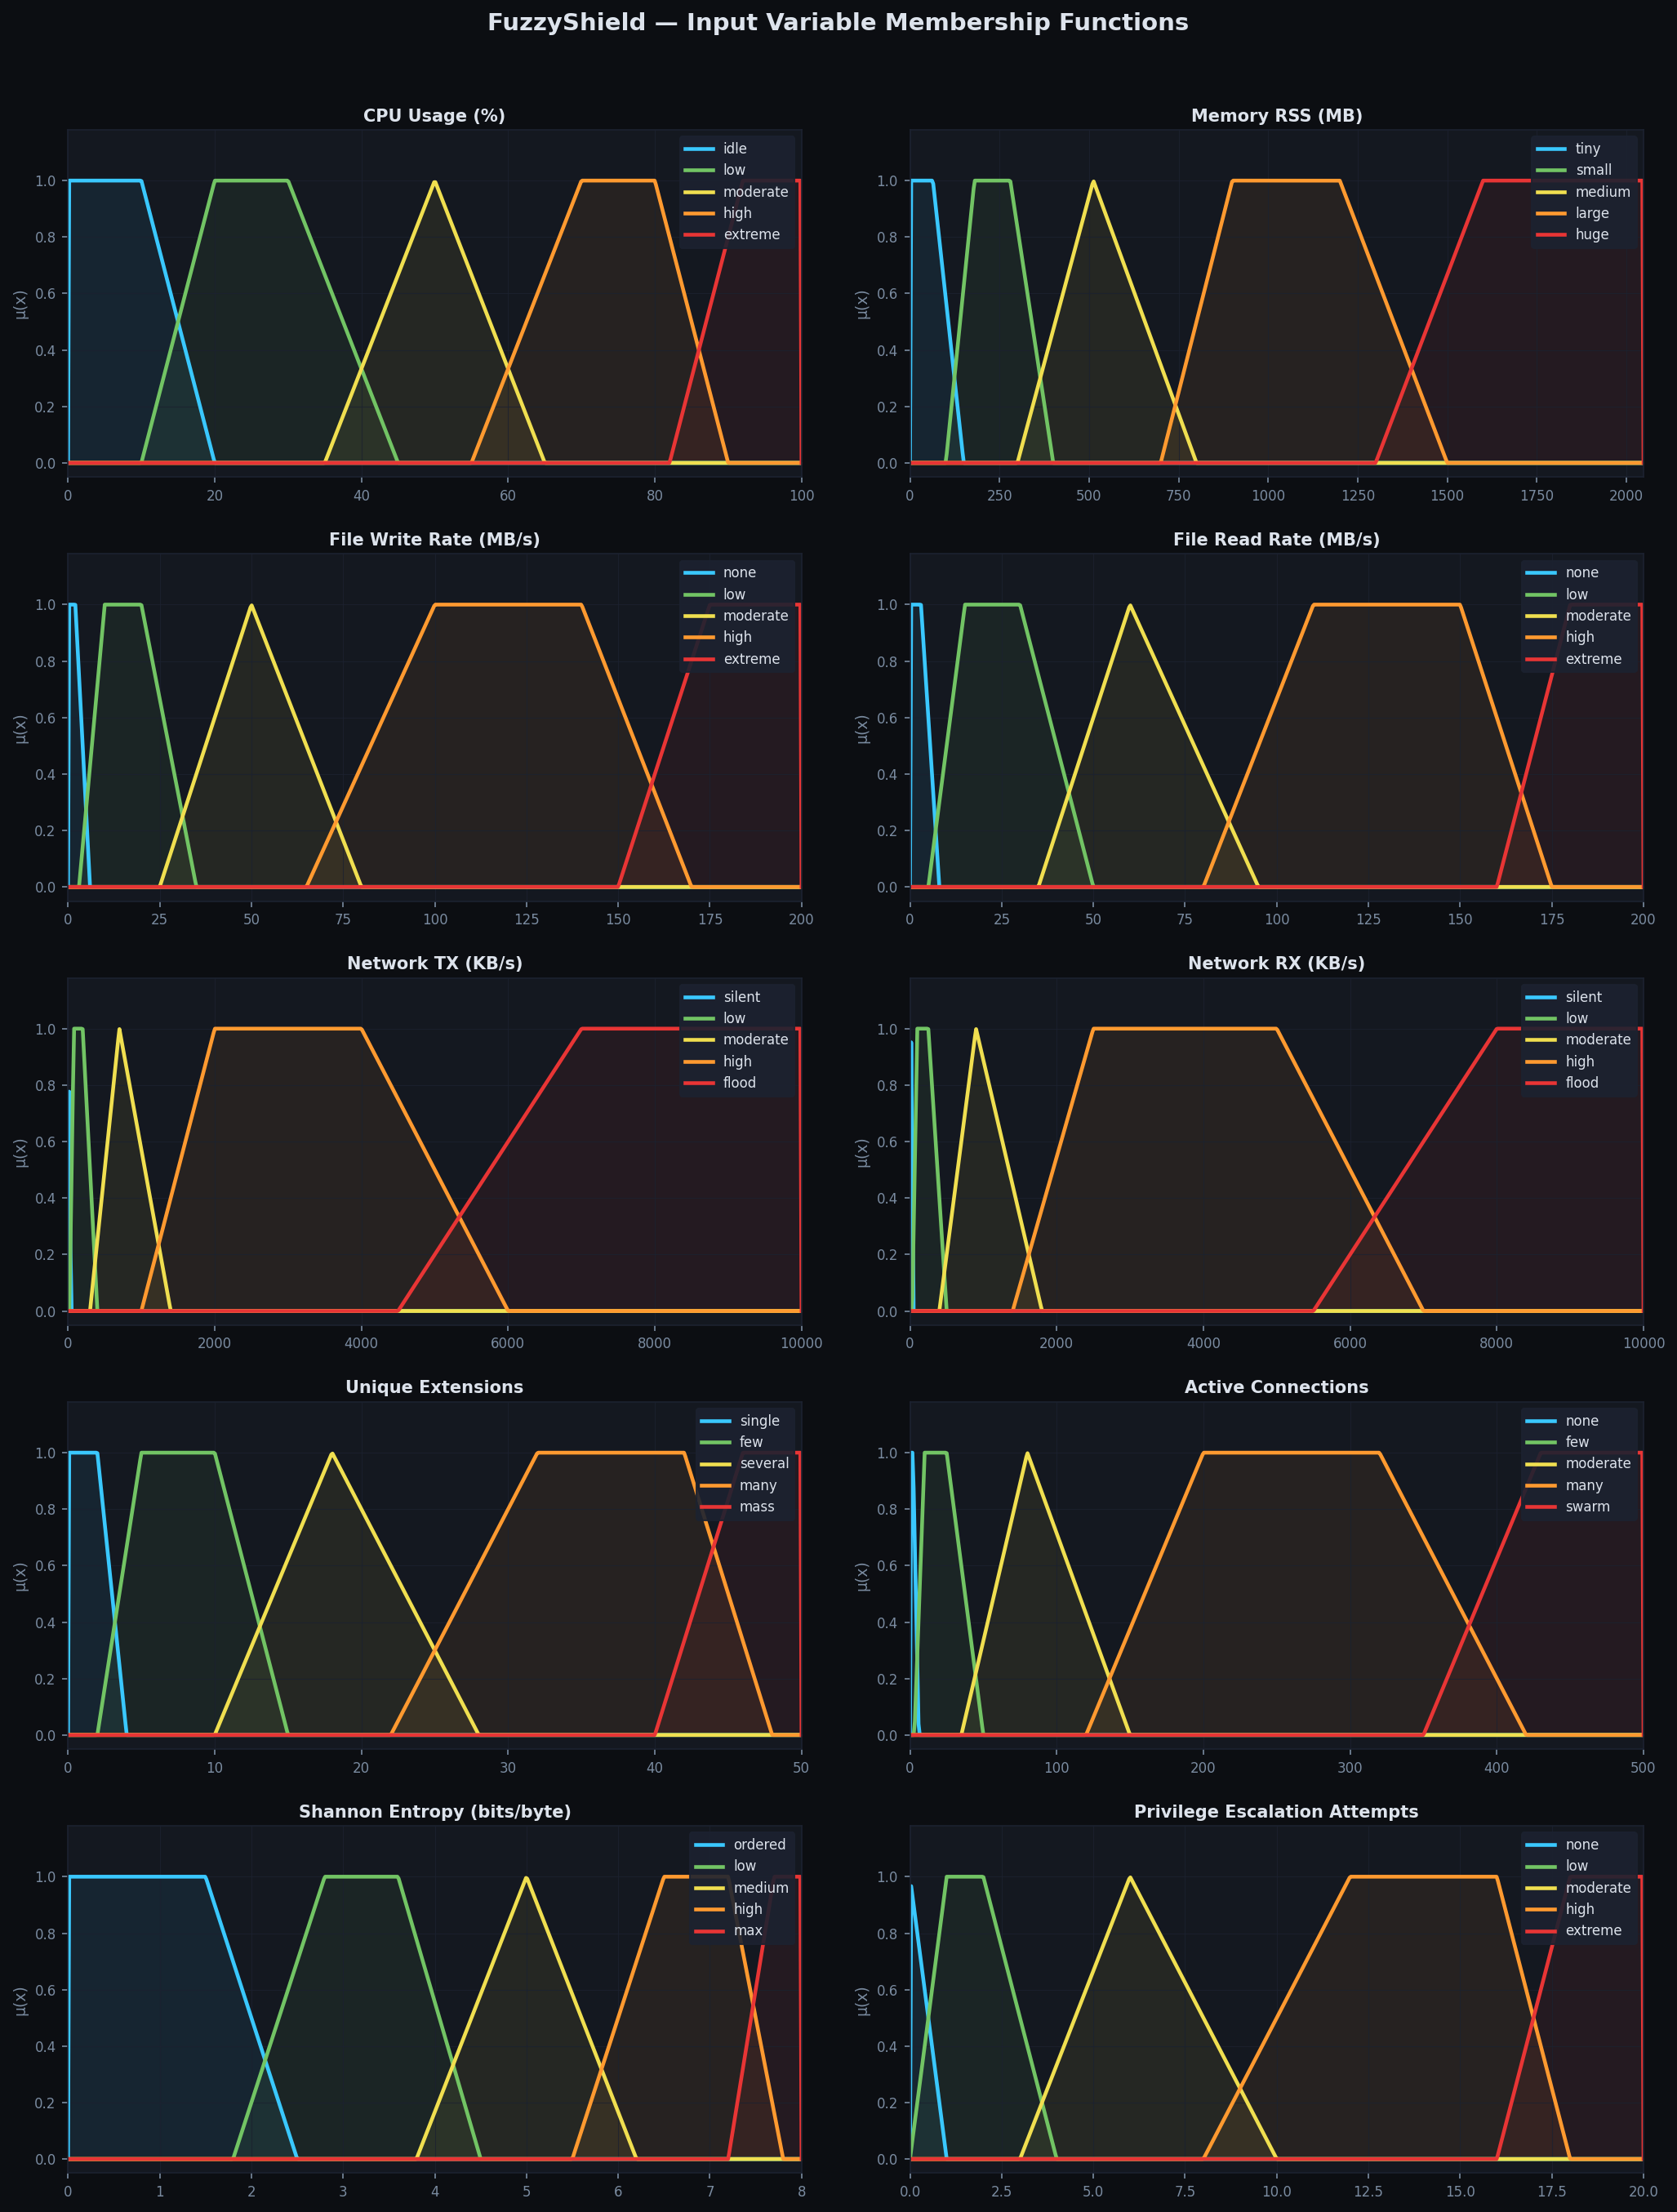
\includegraphics[width=\textwidth]{figures/fig_mf_all_inputs.png}
  \caption{Membership functions for all ten input variables. The five
           linguistic terms (very-low to very-high) overlap to ensure
           smooth fuzzy transitions.}
  \label{fig:mf_all}
\end{figure*}

\begin{figure*}[!t]
  \centering
  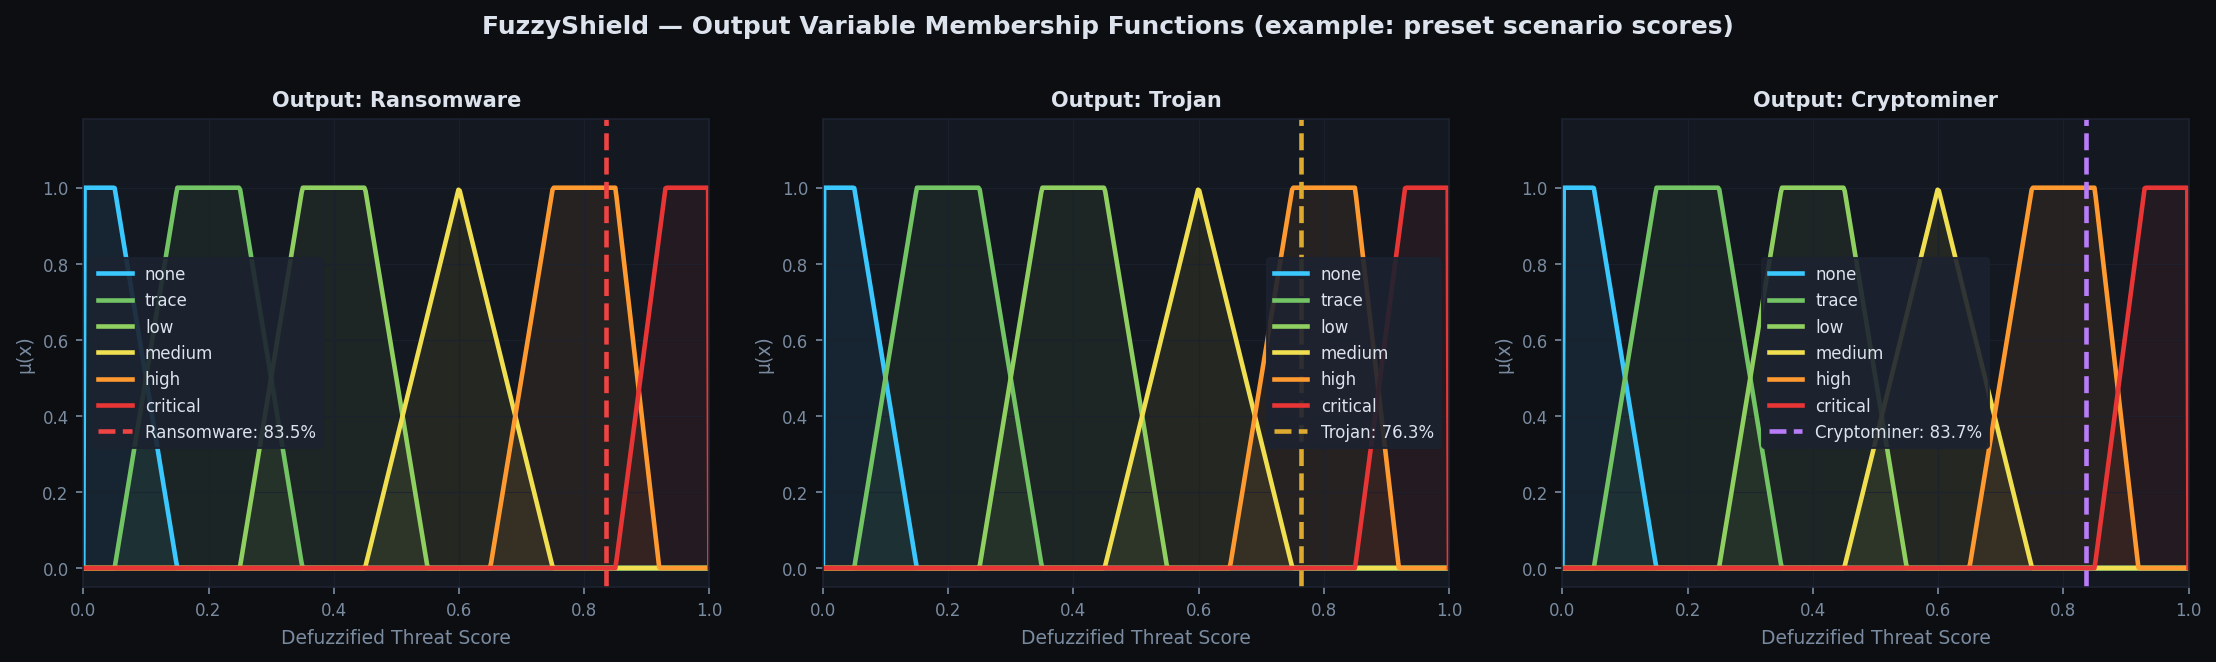
\includegraphics[width=\textwidth]{figures/fig_mf_output.png}
  \caption{Output variable membership functions shown with example
           defuzzified scores for the three preset scenarios.}
  \label{fig:mf_out}
\end{figure*}

\subsection{Rule Base}

FuzzyShield uses 34 Mamdani rules partitioned into five functional
groups. Each rule fires on the AND (min) of its antecedent degrees and
clips the consequent membership functions at the firing strength.

\begin{figure*}[!t]
  \centering
  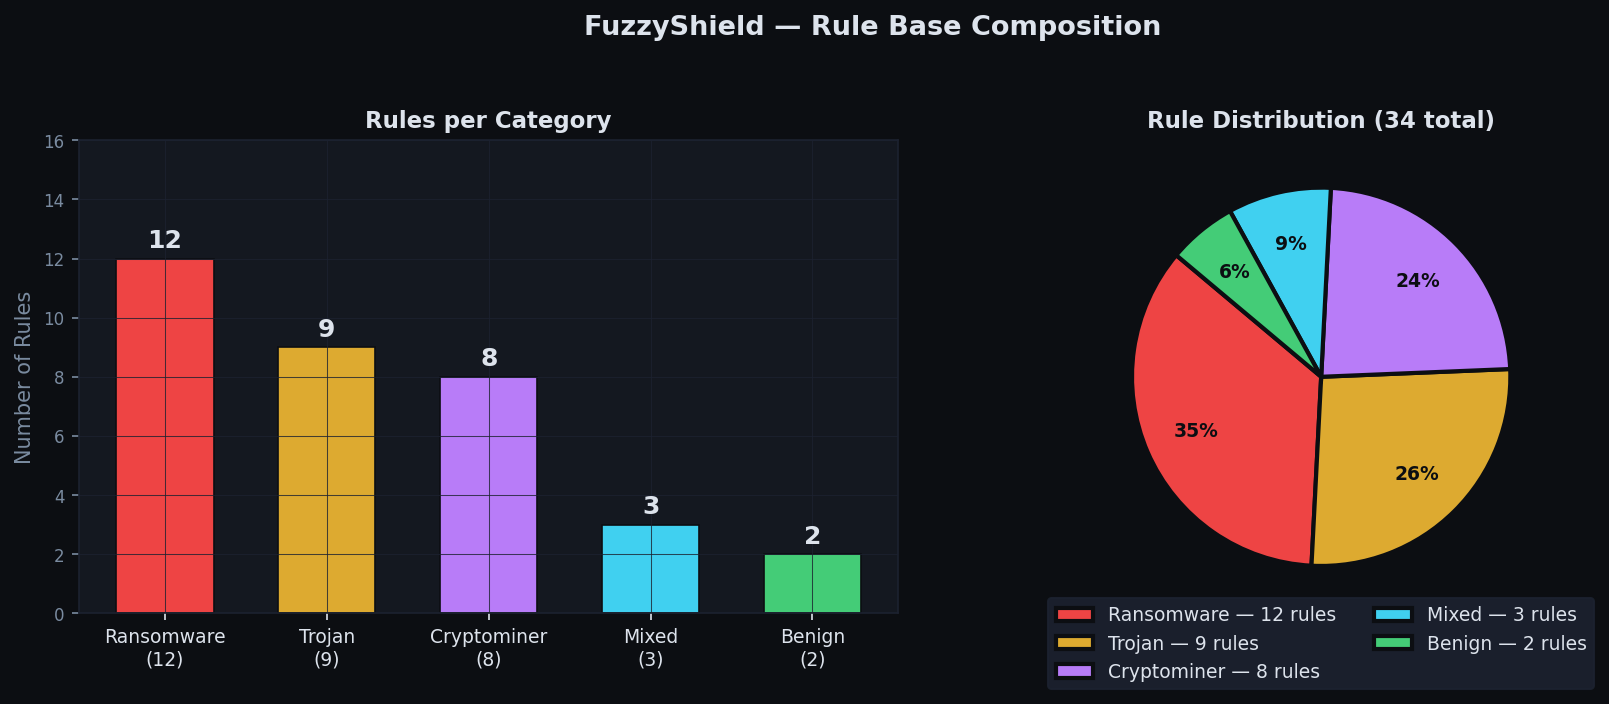
\includegraphics[width=\textwidth]{figures/fig_rule_dist.png}
  \caption{Distribution of 34 rules across threat categories.}
  \label{fig:rule_dist}
\end{figure*}

\subsubsection{Ransomware Rules (12)}

Ransomware rules primarily key on the combination of high write rate,
maximum entropy, and many unique file extensions ---
the \emph{encrypt-and-rename} fingerprint. Representative rules:

\begin{table*}[!t]
\centering
\caption{Selected Ransomware Rules}
\label{tab:ransom_rules}
\small\renewcommand{\arraystretch}{1.2}
\setlength{\tabcolsep}{5pt}
\begin{tabular}{@{} c p{6.0cm} l p{4.5cm} @{}}
\toprule
\textbf{\#} & \textbf{Antecedent} & \textbf{Output} & \textbf{Rationale} \\
\midrule
R1  & fwrite=extreme \& ext=many \& ent=max       & R=critical & strongest encryption signal \\
R2  & fwrite=high \& ext=many \& ent=high         & R=high     & bulk overwrite, many types  \\
R6  & fwrite=high \& ent=max \& priv=moderate     & R=high     & shadow-copy deletion attempt\\
R25 & fwrite=high \& ext=several \& ent=max       & R=high     & crypto burst, fewer types   \\
R27 & fwrite=high \& ent=max \& conn=none         & R=medium   & offline / no C2 encryption  \\
R28 & fwrite=extreme \& fread=low \& ent=max      & R=critical & overwrite without reading   \\
\bottomrule
\end{tabular}
\end{table*}

\subsubsection{Trojan Rules (9)}

Trojan rules focus on high network transmit volume, many simultaneous
connections, and elevated privilege escalation activity:

\begin{table*}[!t]
\centering
\caption{Selected Trojan Rules}
\label{tab:trojan_rules}
\small\renewcommand{\arraystretch}{1.2}
\setlength{\tabcolsep}{5pt}
\begin{tabular}{@{} c p{6.0cm} l p{4.5cm} @{}}
\toprule
\textbf{\#} & \textbf{Antecedent} & \textbf{Output} & \textbf{Rationale} \\
\midrule
R8  & nettx=high \& conn=many \& priv=high    & T=critical & active C2 exfiltration \\
R9  & nettx=flood \& conn=swarm               & T=critical & DDoS or mass-exfiltration \\
R11 & cpu=low \& conn=many \& priv=high       & T=high     & stealthy background trojan\\
R14 & nettx=flood \& priv=extreme             & T=critical & rootkit-level activity \\
R30 & fread=low \& nettx=high \& conn=many    & T=high     & local data, immediate exfil\\
\bottomrule
\end{tabular}
\end{table*}

\subsubsection{Cryptominer Rules (8)}

Cryptominer rules anchor on extreme CPU with negligible file writes and
few persistent connections. The \texttt{conn[few]} condition is critical
to avoid false positives from trojan simulators that also saturate CPU
through many threads:

\begin{table*}[!t]
\centering
\caption{Selected Cryptominer Rules}
\label{tab:crypto_rules}
\small\renewcommand{\arraystretch}{1.2}
\setlength{\tabcolsep}{5pt}
\begin{tabular}{@{} c p{6.8cm} l p{3.8cm} @{}}
\toprule
\textbf{\#} & \textbf{Antecedent} & \textbf{Output} & \textbf{Rationale} \\
\midrule
R16 & cpu=extreme \& fwrite=none \& nettx=moderate          & C=critical & classic SHA-256 miner \\
R17 & cpu=extreme \& mem=large \& nettx=moderate            & C=critical & GPU/DAG miner \\
R19 & cpu=extreme \& fwrite=none \& conn=few \& ent=low     & C=high     & pool protocol, low entropy \\
R22 & cpu=extreme \& fwrite=none \& conn=few                & C=high     & offline miner (no pool) \\
R24 & cpu=extreme \& fwrite=none \& conn=few \& ent=ordered & C=critical & strongest offline fingerprint \\
\bottomrule
\end{tabular}
\end{table*}

\subsubsection{Mixed Rules (3)}

Three rules explicitly model ambiguous behaviors that fit multiple
categories:

\begin{itemize}[leftmargin=2em]
  \item \textbf{M1}: cpu=high \& fwrite=high \& nettx=high
        $\rightarrow$ R=medium, T=medium, C=trace
        (high resource usage across all channels)
  \item \textbf{M2}: priv=moderate \& ent=high \& nettx=moderate
        $\rightarrow$ R=medium, T=medium, C=trace
        (ambiguous privilege + encryption behavior)
  \item \textbf{M3}: priv=extreme \& ent=max \& conn=many
        $\rightarrow$ R=high, T=high
        (simultaneous ransomware-level encryption and trojan-level networking)
\end{itemize}

\subsubsection{Benign Rules (2)}

Two benign rules suppress false positives for idle or normal processes:
\begin{itemize}[leftmargin=2em]
  \item \textbf{B1}: cpu=idle \& fwrite=none \& nettx=silent \& conn=none
        $\rightarrow$ all outputs = none
  \item \textbf{B2}: cpu=idle \& ext=single \& ent=ordered \& priv=none
        $\rightarrow$ all outputs = none
\end{itemize}

\subsection{Defuzzification and Verdict Generation}

The centroid defuzzifier integrates the aggregated output fuzzy set over
the $[0,1]$ output domain to produce a crisp threat score for each
channel. The verdict module then applies the following logic:

\begin{enumerate}[leftmargin=2em]
  \item If $\max(R, T, C) < 0.10$: verdict = \textbf{BENIGN} (SAFE).
  \item If $\max(R, T, C) < 0.40$: verdict = \textbf{SUSPICIOUS} (INCONCLUSIVE).
  \item Otherwise, collect all channels with score
        $\geq \max - \Delta_{\text{tie}}$ and score $\geq \theta_{\text{min}}$,
        where $\Delta_{\text{tie}} = 0.05$ and $\theta_{\text{min}} = 0.35$.
        Join active threat names with ``$+$'' for compound verdicts.
  \item If $\max < 0.70$: confidence = LIKELY THREAT; else HIGH CONFIDENCE.
\end{enumerate}

This design prevents a single dominant channel from masking a
co-occurring threat that scores within $5\%$ of the maximum.

\subsection{Temporal Score Smoothing (Asymmetric EWMA)}
\label{sec:ewma}

In real-time PID monitoring, a single noisy measurement window can
transiently suppress a malware score or allow a malware process to
temporarily idle below the detection threshold. The
\texttt{EWMAFeedback} module addresses both problems by applying an
asymmetric exponential weighted moving average to the FIS output at each
check.

Let $s_t$ be the raw defuzzified score at check $t$ and $\hat{s}_{t-1}$
the smoothed score from the previous check (initialised to $0$). The
update rule is the standard first-order EWMA:
\[
  \hat{s}_t \;=\; \alpha\,\hat{s}_{t-1} + (1-\alpha)\,s_t
\]
The smoothing coefficient $\alpha$ is chosen based on the direction of
change:
\[
  \alpha = \begin{cases}
    \alpha_{\uparrow} = 0.15 & \text{if } s_t \geq \hat{s}_{t-1}
                               \quad\text{(score rising)}\\[4pt]
    \alpha_{\downarrow} = 0.85 & \text{if } s_t < \hat{s}_{t-1}
                               \quad\text{(score falling)}
  \end{cases}
\]

When $\alpha_{\uparrow}=0.15$ the new observation receives weight
$(1{-}0.15)=0.85$, so a fresh threat signal dominates the smoothed score
within a single window and alarms are not delayed. When
$\alpha_{\downarrow}=0.85$ the previous smoothed score retains weight
$0.85$ and the new (quieter) value contributes only $0.15$, so a single
idle window cannot reset an active alarm. This asymmetry neutralises
\emph{burst-pause evasion}, where malware alternates short bursts of
malicious I/O or CPU activity with idle intervals timed to confuse
one-window detectors.

The verdict is always computed on $\hat{s}_t$ (the smoothed score), not
on the raw $s_t$. The rolling time-series dashboard plots both raw
(dashed, semi-transparent) and smoothed (solid) series so that the
feedback effect is immediately visible to the analyst.

% ════════════════════════════════════════════════════════════════════════════
\section{Implementation}

The complete source code of both implementations, the behavioral
simulator, and usage guidelines are publicly available in the project
repository.\footnote{\url{https://github.com/Farukesgin/FuzzyShield}}

\subsection{Python Implementation}

The Python implementation uses \texttt{scikit-fuzzy}
(version~0.4.2)~\cite{warner2019skfuzzy}, a NumPy-based fuzzy logic
library. The FIS is defined using the \texttt{skfuzzy.control} API:

\begin{lstlisting}[language=Python, caption={Example rule definition in Python
(scikit-fuzzy)}, label={lst:rule}]
import skfuzzy as fuzz
import skfuzzy.control as ctrl

# Antecedent (input) and Consequent (output) definitions
cpu       = ctrl.Antecedent(np.arange(0, 101, 0.5), 'cpu')
fwrite    = ctrl.Antecedent(np.arange(0, 201, 0.5), 'fwrite')
ent       = ctrl.Antecedent(np.arange(0, 8.1, 0.05), 'ent')
ransomware = ctrl.Consequent(np.arange(0, 1.01, 0.005), 'ransomware')

# Membership function assignment
cpu['extreme'] = fuzz.trapmf(cpu.universe, [82, 92, 100, 100])
fwrite['extreme'] = fuzz.trapmf(fwrite.universe, [150, 175, 200, 200])
ent['max'] = fuzz.trapmf(ent.universe, [7.2, 7.7, 8.0, 8.0])
ransomware['critical'] = fuzz.trapmf(ransomware.universe, [0.85, 0.93, 1.0, 1.0])

# Rule definition
rule_R1 = ctrl.Rule(
    fwrite['extreme'] & ext['many'] & ent['max'],
    (ransomware['critical'], trojan['none'], cryptominer['none'])
)
\end{lstlisting}

The \texttt{ControlSystem} object is created once at startup; subsequent
calls reuse the compiled structure by resetting the
\texttt{ControlSystemSimulation} inputs, minimising per-inference
overhead. Process metrics are collected with \texttt{psutil.Process},
using \texttt{/proc/pid/io} \texttt{wchar} (write characters) rather
than \texttt{write\_bytes} to capture all user-space writes including
buffered I/O.

The monitoring loop samples metrics over an interval $\Delta t$, computes
rates (MB/s, KB/s), feeds the vector to the FIS, and saves timestamped
PNG plots to an organised \texttt{output/} directory hierarchy:
\texttt{output/scenarios/}, \texttt{output/pid\_sessions/},
and \texttt{output/analysis/}.

\subsection{MATLAB Implementation}

An exact mirror of the rule base is implemented in MATLAB using the Fuzzy
Logic Toolbox \texttt{mamfis} API. The \texttt{fuzzy\_shield.m} script
programmatically constructs the FIS, adds all 34 rules via
\texttt{addRule}, evaluates scenarios with \texttt{evalfis}, and exports
the FIS to \texttt{FuzzyShield.fis} for use in the Fuzzy Logic Designer
GUI.

The MATLAB rule array encodes each rule as a 15-column integer vector:
columns 1--10 specify input MF indices (0 = don't care), columns 11--13
specify output MF indices, column~14 is the rule weight (always~1), and
column~15 is the AND connector (1~=~min T-norm). Both implementations use
identical membership function parameters, ensuring numerical output
agreement.

\subsection{Behavioral Malware Simulator}

\texttt{sim/malware\_sim.py} generates authentic behavioral signals for
each malware type on the local machine without touching system files or
external networks:

\begin{itemize}[leftmargin=2em]
  \item \textbf{Ransomware}: 8 concurrent worker threads each write
        500 KB of \texttt{os.urandom()} bytes to randomly named files
        in \texttt{/tmp/}, cycling through 20 file extensions. Files are
        held open for 40 ms to ensure \texttt{psutil.open\_files()} can
        sample the extension set.
  \item \textbf{Trojan}: 250 persistent loopback TCP connections to a
        local echo server each send 2 KB payloads at 50 sends/second,
        producing $\approx$25 MB/s TX/RX.
  \item \textbf{Cryptominer}: $N_{\text{cores}}$ SHA-256 hashing threads
        saturate all CPU cores; 8 pool-talker threads maintain binary
        protocol connections ($\approx$640 KB/s TX).
  \item \textbf{Benign}: idle sleep loop, minimal resource use.
\end{itemize}

% ════════════════════════════════════════════════════════════════════════════
\section{Experimental Results}

\subsection{Scenario-Based Evaluation}

Five preset input vectors were evaluated to validate the rule base.
Table~\ref{tab:inputs_all} lists the crisp input values for each
scenario, and Figure~\ref{fig:results} shows the defuzzified output
scores.

\begin{table*}[!t]
\centering
\caption{Scenario Input Vectors}
\label{tab:inputs_all}
\renewcommand{\arraystretch}{1.2}
\small\setlength{\tabcolsep}{4pt}
\begin{tabular}{@{} l r r r r r r r r r r @{}}
\toprule
\textbf{Scenario} & \textbf{cpu} & \textbf{mem} & \textbf{fwrite} & \textbf{fread} & \textbf{nettx} & \textbf{netrx} & \textbf{ext} & \textbf{conn} & \textbf{ent} & \textbf{priv} \\
 & \% & MB & MB/s & MB/s & KB/s & KB/s & & & bits/B & \\
\midrule
Ransomware  & 75 & 480  & 160 & 40 & 80   & 50   & 45 & 12  & 7.8 & 3  \\
Trojan      & 18 & 210  & 8   & 12 & 4200 & 3500 & 5  & 320 & 3.2 & 14 \\
Cryptominer & 96 & 1400 & 2   & 5  & 600  & 200  & 2  & 20  & 2.8 & 1  \\
Benign      & 12 & 180  & 4   & 8  & 60   & 90   & 3  & 4   & 2.1 & 0  \\
Mixed$^{\dagger}$ & 75 & 550 & 170 & 45 & 1800 & 1500 & 38 & 180 & 7.8 & 10 \\
\bottomrule
\end{tabular}

\smallskip
{\footnotesize $^{\dagger}$The mixed preset generates
  randomised inputs within defined overlap ranges each run; values shown
  are a fixed illustrative example.}
\end{table*}

\begin{table*}[!t]
\centering
\caption{FIS Output Scores and Verdicts}
\label{tab:output_scores}
\small\renewcommand{\arraystretch}{1.25}
\setlength{\tabcolsep}{5pt}
\begin{tabular}{@{} l c c c p{4.2cm} p{3.4cm} @{}}
\toprule
\textbf{Scenario} & \textbf{R (\%)} & \textbf{T (\%)} & \textbf{C (\%)} &
\textbf{Verdict} & \textbf{Confidence} \\
\midrule
Ransomware  & \textbf{83.5} & 14.1 &  6.6 & RANSOMWARE            & HIGH CONFIDENCE \\
Trojan      & 15.7 & \textbf{76.3} & 15.7 & TROJAN                & HIGH CONFIDENCE \\
Cryptominer &  5.4 &  5.4 & \textbf{83.7} & CRYPTOMINER           & HIGH CONFIDENCE \\
Benign      &  6.6 &  6.6 &  6.6          & BENIGN                & SAFE \\
Mixed       & \textbf{50.6} & \textbf{51.0} & 9.0 &
    \textbf{RANSOMWARE + TROJAN} & LIKELY THREAT \\
\bottomrule
\end{tabular}
\end{table*}

\begin{figure*}[!t]
  \centering
  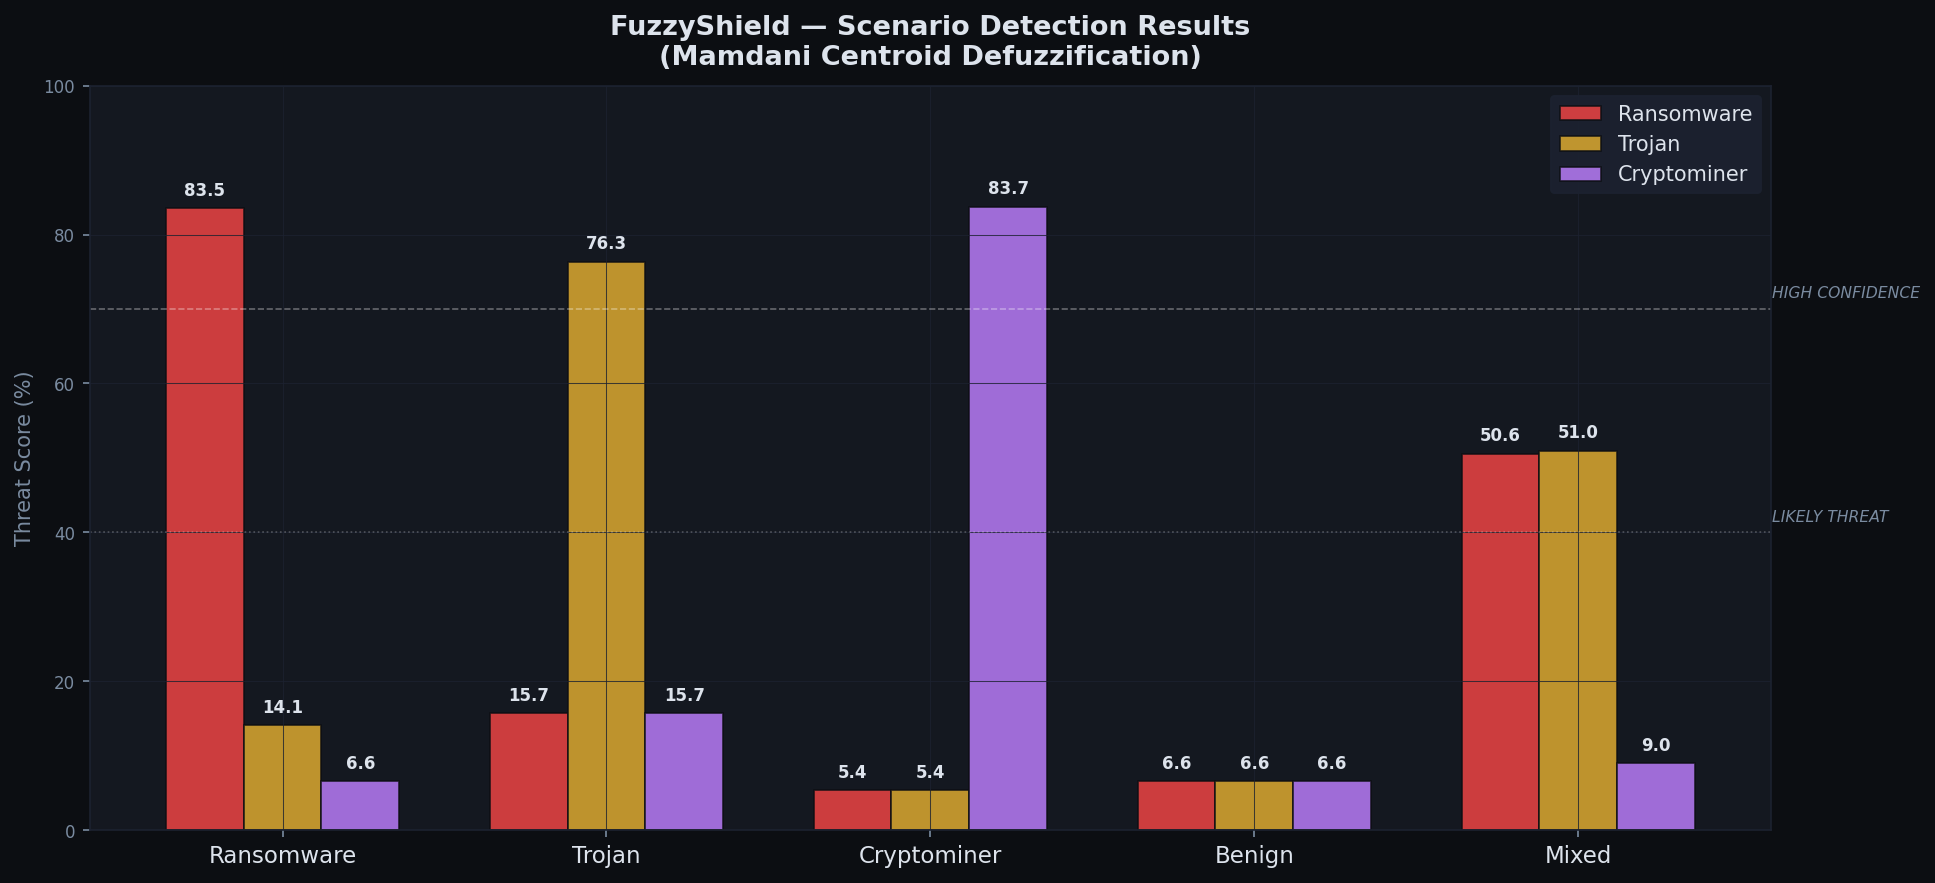
\includegraphics[width=\textwidth]{figures/fig_results.png}
  \caption{Defuzzified threat scores for all five test scenarios.
           Dashed lines mark the LIKELY THREAT (40\%) and
           HIGH CONFIDENCE (70\%) thresholds.}
  \label{fig:results}
\end{figure*}

All four single-threat scenarios are classified with high confidence:
\begin{itemize}[leftmargin=2em]
  \item \textbf{Ransomware} (83.5\%): Rules R1, R2, R5, R25--R28 fire.
        fwrite=160 MB/s (extreme), ext=45 (mass), ent=7.8 (max) trigger
        the strongest ransomware antecedents.
  \item \textbf{Trojan} (76.3\%): Rules R8, R9, R10, R12 fire.
        nettx=4200 KB/s (high), conn=320 (many), priv=14 (high) activate
        the critical-tier trojan rules.
  \item \textbf{Cryptominer} (83.7\%): Rules R16, R17, R20, R22 fire.
        cpu=96\% (extreme), mem=1400 MB (huge), fwrite=2 MB/s (none),
        conn=20 (few), nettx=600 KB/s (moderate).
  \item \textbf{Benign} (6.6\%): Benign rules B1 and B2 suppress all
        threat channels. Score below 10\% triggers the SAFE verdict.
\end{itemize}

\subsection{Compound Threat Detection}

The mixed scenario demonstrates the compound-verdict capability. With
fwrite=170 MB/s (extreme) and ent=7.8 (max), ransomware rules fire at
full strength; simultaneously, nettx=1800 KB/s (high), conn=180 (many),
and priv=10 (high) activate trojan rules. Mixed rule M3 (priv=extreme,
ent=max, conn=many) also contributes to both channels.

The result --- R=50.6\%, T=51.0\% --- places both threats within the
$\Delta_{\text{tie}} = 5\%$ window and above $\theta_{\text{min}} = 35\%$,
triggering the \textbf{RANSOMWARE + TROJAN} compound verdict with two
independent remediation recommendations issued to the analyst.

\begin{figure*}[!t]
  \centering
  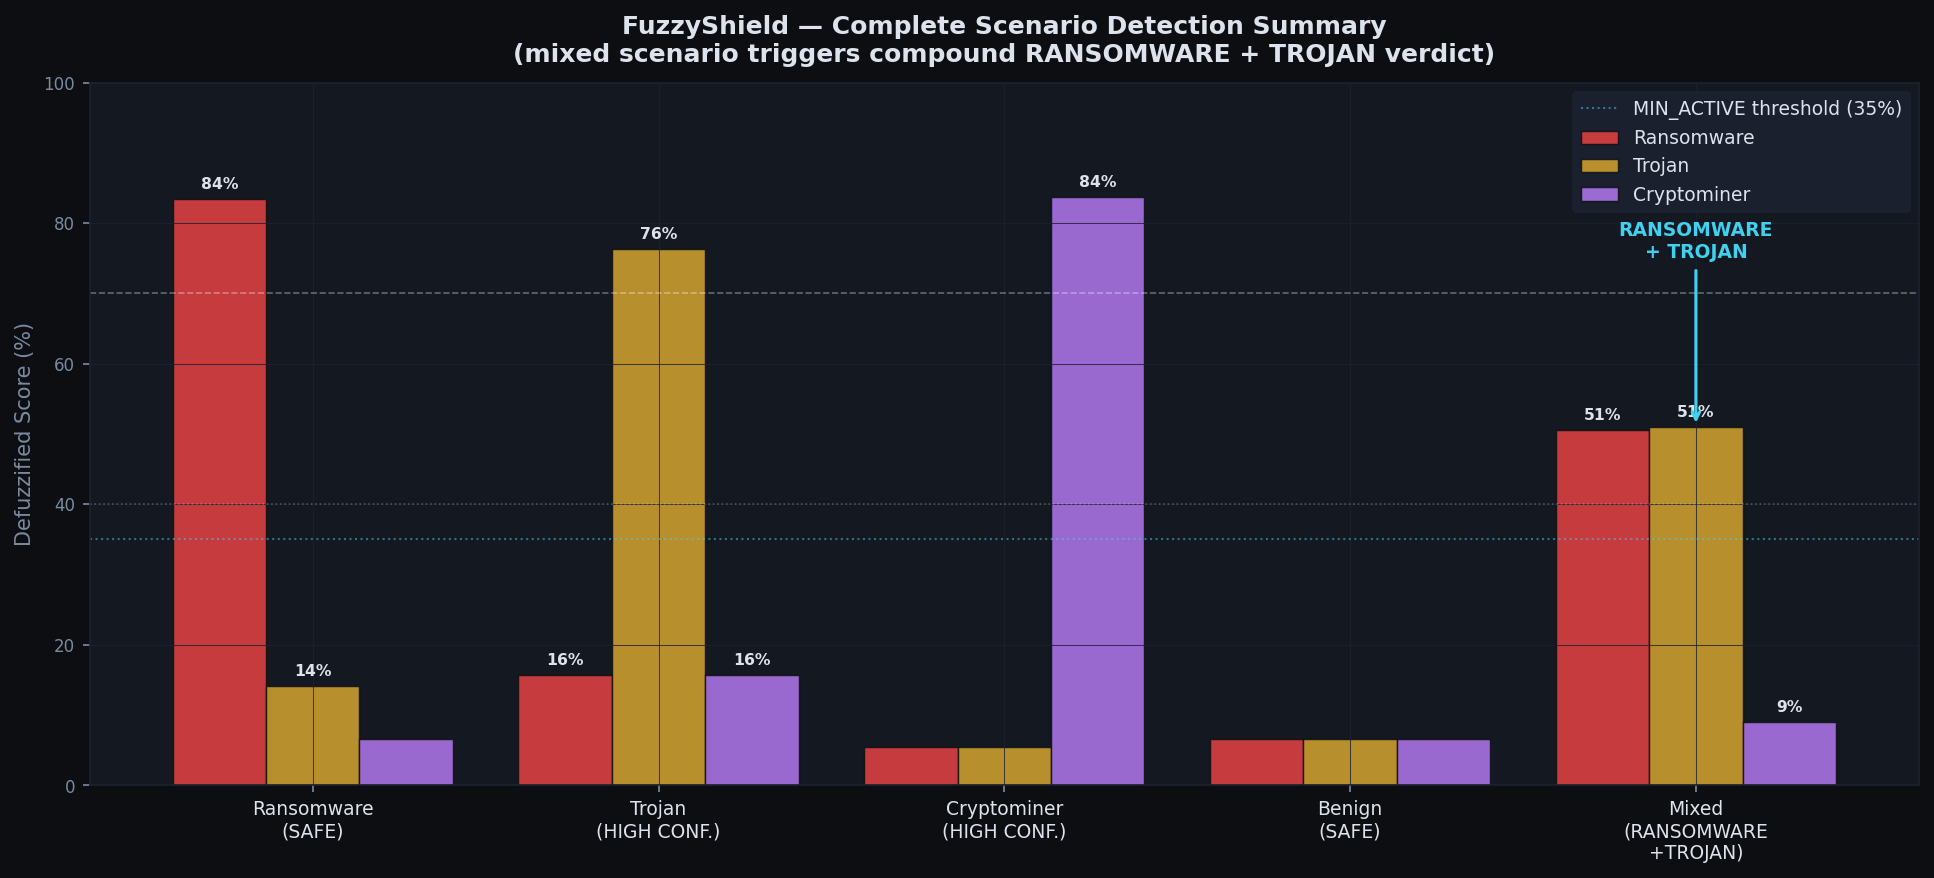
\includegraphics[width=\textwidth]{figures/fig_compound.png}
  \caption{Complete scenario detection summary. The mixed scenario
           (rightmost group) activates both Ransomware and Trojan
           channels above the minimum active threshold, producing a
           compound verdict.}
  \label{fig:compound}
\end{figure*}

\subsection{Rule Surface Analysis}

Figure~\ref{fig:surfaces} shows six 3D rule surface plots computed by
sweeping two input dimensions while holding the remaining eight fixed at
benign defaults. These surfaces visualise how the Mamdani inference
maps input combinations to output probabilities.

\begin{figure*}[!t]
  \centering
  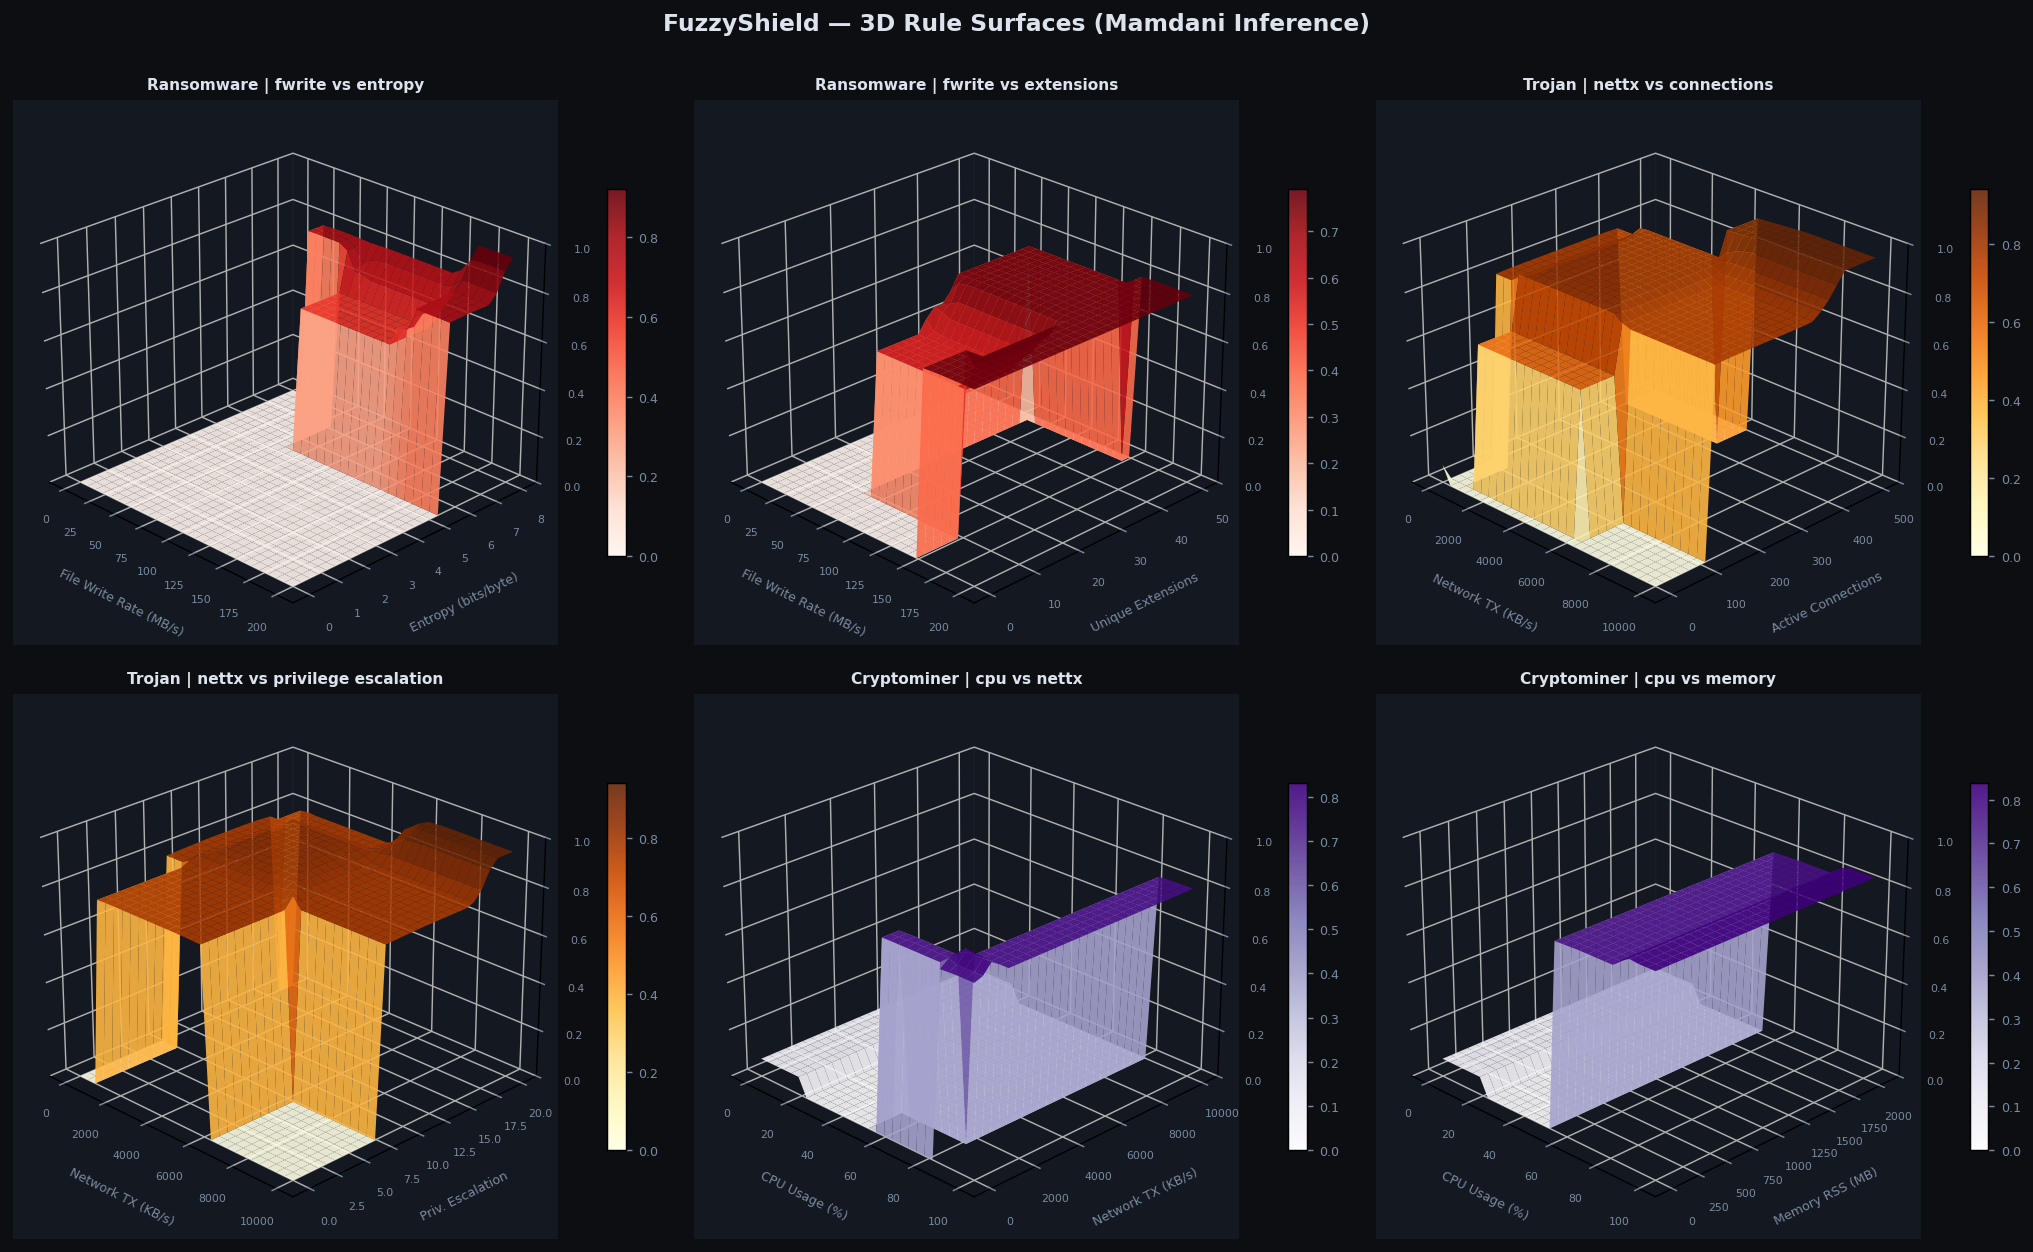
\includegraphics[width=\textwidth]{figures/fig_surfaces.png}
  \caption{3D rule surfaces. Top row: Ransomware output vs.\ (fwrite,
           entropy) and (fwrite, extensions). Middle row: Trojan output
           vs.\ (nettx, connections) and (nettx, privilege). Bottom row:
           Cryptominer output vs.\ (cpu, nettx) and (cpu, memory).}
  \label{fig:surfaces}
\end{figure*}

Key observations:
\begin{itemize}[leftmargin=2em]
  \item The ransomware surface rises sharply when both fwrite and entropy
        exceed their ``high'' transition zones simultaneously, confirming
        that neither metric alone is sufficient.
  \item The trojan surface shows a plateau region at high nettx and high
        conn, where multiple trojan rules overlap and aggregate to
        near-critical scores.
  \item The cryptominer surface reveals a narrow ridge along the
        cpu=extreme axis with moderate nettx, reflecting the tight
        constraint that miners use \emph{all} CPU cores but only
        \emph{moderate} network bandwidth.
\end{itemize}

\subsection{Real-Time PID Monitoring}

The system was validated by monitoring live instances of
\texttt{sim/malware\_sim.py}. Each monitored session samples metrics
every 5 seconds for 6 checks and saves:
\begin{itemize}[leftmargin=2em]
  \item Per-check membership function plots (\texttt{checkNN\_membership.png})
  \item Per-check results dashboard (\texttt{checkNN\_results.png})
  \item A rolling time-series chart (\texttt{timeseries.png})
\end{itemize}
All outputs are timestamped and stored under
\texttt{output/pid\_sessions/} in per-session sub-folders named
\texttt{<timestamp>\_pid<N>\_<name>}.

The asymmetric EWMA feedback module (Section~\ref{sec:ewma}) is active
throughout each monitoring session. At every check, the raw FIS scores
are smoothed before the verdict is issued; both raw (dashed) and smoothed
(solid) series appear in the time-series dashboard, making the feedback
effect directly observable.

The ransomware simulator consistently produced a smoothed R $\geq 70\%$
within the first check due to the fast $\alpha_{\uparrow}=0.15$ rise
response; the cryptominer required 2--3 checks for the CPU metric to
fully stabilise at the extreme level. Once triggered, the
$\alpha_{\downarrow}=0.85$ fall coefficient kept scores elevated even
during a brief simulated idle window, confirming resistance to burst-pause
evasion.

% ════════════════════════════════════════════════════════════════════════════
\section{Conclusion}

This project presented FuzzyShield, a real-time behavioral malware
classifier based on a 10-input, 3-output Mamdani fuzzy inference system.
The system successfully classifies Ransomware, Trojan, and Cryptominer
with high confidence on preset scenarios, and gracefully handles
ambiguous mixed-threat inputs through a compound verdict mechanism.
An asymmetric EWMA temporal feedback layer ($\alpha_{\uparrow}=0.15$,
$\alpha_{\downarrow}=0.85$) stabilises real-time scores against
measurement noise and burst-pause evasion without delaying legitimate
alarms. The identical rule base shared between the Python and MATLAB
implementations ensures cross-platform reproducibility and facilitates
verification in both research and educational settings.

\subsubsection*{Limitations}

Behavioural metrics are inherently noisy.  The primary false-positive
risk arises from processes that combine moderate-to-high CPU utilisation,
moderate outbound network traffic, and a low file-write rate---the exact
signature targeted by rules~R18 and R21.  Lightweight web servers serving
cached content (high CPU, moderate TX, near-zero writes) sit at the
boundary of the SUSPICIOUS/LIKELY~THREAT verdict.  Rules~R18 and R21
include an explicit \texttt{fwrite\,=\,none} guard to exclude
write-intensive processes (update daemons, compilers, databases), but a
web server whose write rate genuinely approaches zero remains ambiguous
and requires temporal confirmation.  In real-time monitoring mode the
asymmetric EWMA mitigates this: a true cryptominer sustains its signal
across consecutive windows, whereas a web server's CPU and traffic load
fluctuates with request patterns.  In single-shot scenario mode the raw
score from one window is used directly, so an isolated anomalous
measurement can still produce a spurious alert; extending evaluations to
5--10 consecutive checks before acting is recommended.  The current
entropy measurement reads recently written file tails and may miss write
buffers flushed asynchronously.

\subsubsection*{Future Work}

\begin{itemize}[leftmargin=2em]
  \item \textbf{Adaptive rule base}: use reinforcement learning to
        tune membership function parameters automatically from labelled
        malware samples.
  \item \textbf{Extended temporal features}: supplement the existing
        asymmetric EWMA feedback with trend-based statistics (entropy
        slope, connection rate of change) as dedicated FIS input variables
        to detect slow-ramping ransomware variants that evade even
        persistent EWMA signals.
  \item \textbf{Kernel integration}: replace \texttt{psutil} with eBPF
        probes for lower-latency, tamper-resistant metric collection.
  \item \textbf{Wider malware taxonomy}: extend outputs to cover worms,
        rootkits, and adware.
\end{itemize}

% ════════════════════════════════════════════════════════════════════════════
\begin{thebibliography}{99}

\bibitem{zadeh1965}
L.~A. Zadeh,
``Fuzzy sets,''
\textit{Information and Control}, vol.~8, no.~3, pp.~338--353, 1965.

\bibitem{mamdani1975}
E.~H. Mamdani and S.~Assilian,
``An experiment in linguistic synthesis with a fuzzy logic controller,''
\textit{International Journal of Man-Machine Studies}, vol.~7, no.~1,
pp.~1--13, 1975.

\bibitem{kharaz2016unveil}
A.~Kharaz, S.~Arshad, C.~Mulliner, W.~Robertson, and E.~Kirda,
``UNVEIL: A large-scale, automated approach to detecting ransomware,''
in \textit{Proc. 25th USENIX Security Symposium}, 2016, pp.~757--772.

\bibitem{egele2012survey}
M.~Egele, T.~Scholte, E.~Kirda, and C.~Kruegel,
``A survey on automated dynamic malware-analysis techniques and tools,''
\textit{ACM Computing Surveys}, vol.~44, no.~2, pp.~1--42, 2012.

\bibitem{gomes2021detecting}
C.~Gomes, M.~In\'{a}cio, and M.~Freire,
``Detecting cryptomining on endpoints using resource-usage profiling,''
\textit{IEEE Access}, vol.~9, pp.~70088--70107, 2021.

\bibitem{kolbitsch2009}
C.~Kolbitsch, P.~Comparetti, C.~Kruegel, E.~Kirda, X.~Zhou, and X.~Wang,
``Effective and efficient malware detection at the end host,''
in \textit{Proc. 18th USENIX Security Symposium}, 2009, pp.~351--366.

\bibitem{rieck2011}
K.~Rieck, P.~Trinius, C.~Willems, and T.~Holz,
``Automatic analysis of malware behavior using machine learning,''
\textit{Journal of Computer Security}, vol.~19, no.~4,
pp.~639--668, 2011.

\bibitem{alazab2012}
M.~Alazab, S.~Venkataraman, and P.~Watters,
``Towards understanding malicious behaviour by visualizing malware
forensics,''
in \textit{Proc. 6th IEEE International Workshop on Visualization for
Cyber Security}, 2012, pp.~1--11.

\bibitem{mosli2017}
R.~Mosli, R.~Li, B.~Yuan, and Y.~Pan,
``Automated malware detection using artifacts in forensic memory images,''
in \textit{Proc. IEEE IPCCC}, 2017, pp.~1--8.

\bibitem{warner2019skfuzzy}
J.~D. Warner \textit{et al.},
``scikit-fuzzy: A fuzzy logic toolkit for SciPy,''
\textit{Journal of Open Source Software}, vol.~4, no.~35, p.~1234, 2019.

\end{thebibliography}

\end{document}
